\documentclass{article}
\usepackage[utf8]{inputenc}
\title{MATH 20C Notes - Week Six}
\author{C-Rin}
\date{October 2019}

\usepackage{natbib}
\usepackage{graphicx}
\usepackage{gensymb}
\usepackage{amsmath}
\usepackage{amssymb}
\usepackage{wrapfig}
\usepackage{diffcoeff}
\usepackage{microtype}

\graphicspath{ {./images/} }

\begin{document}

\maketitle

\section*{Introduction}
Deep 

\begin{figure}[h!]
\centering
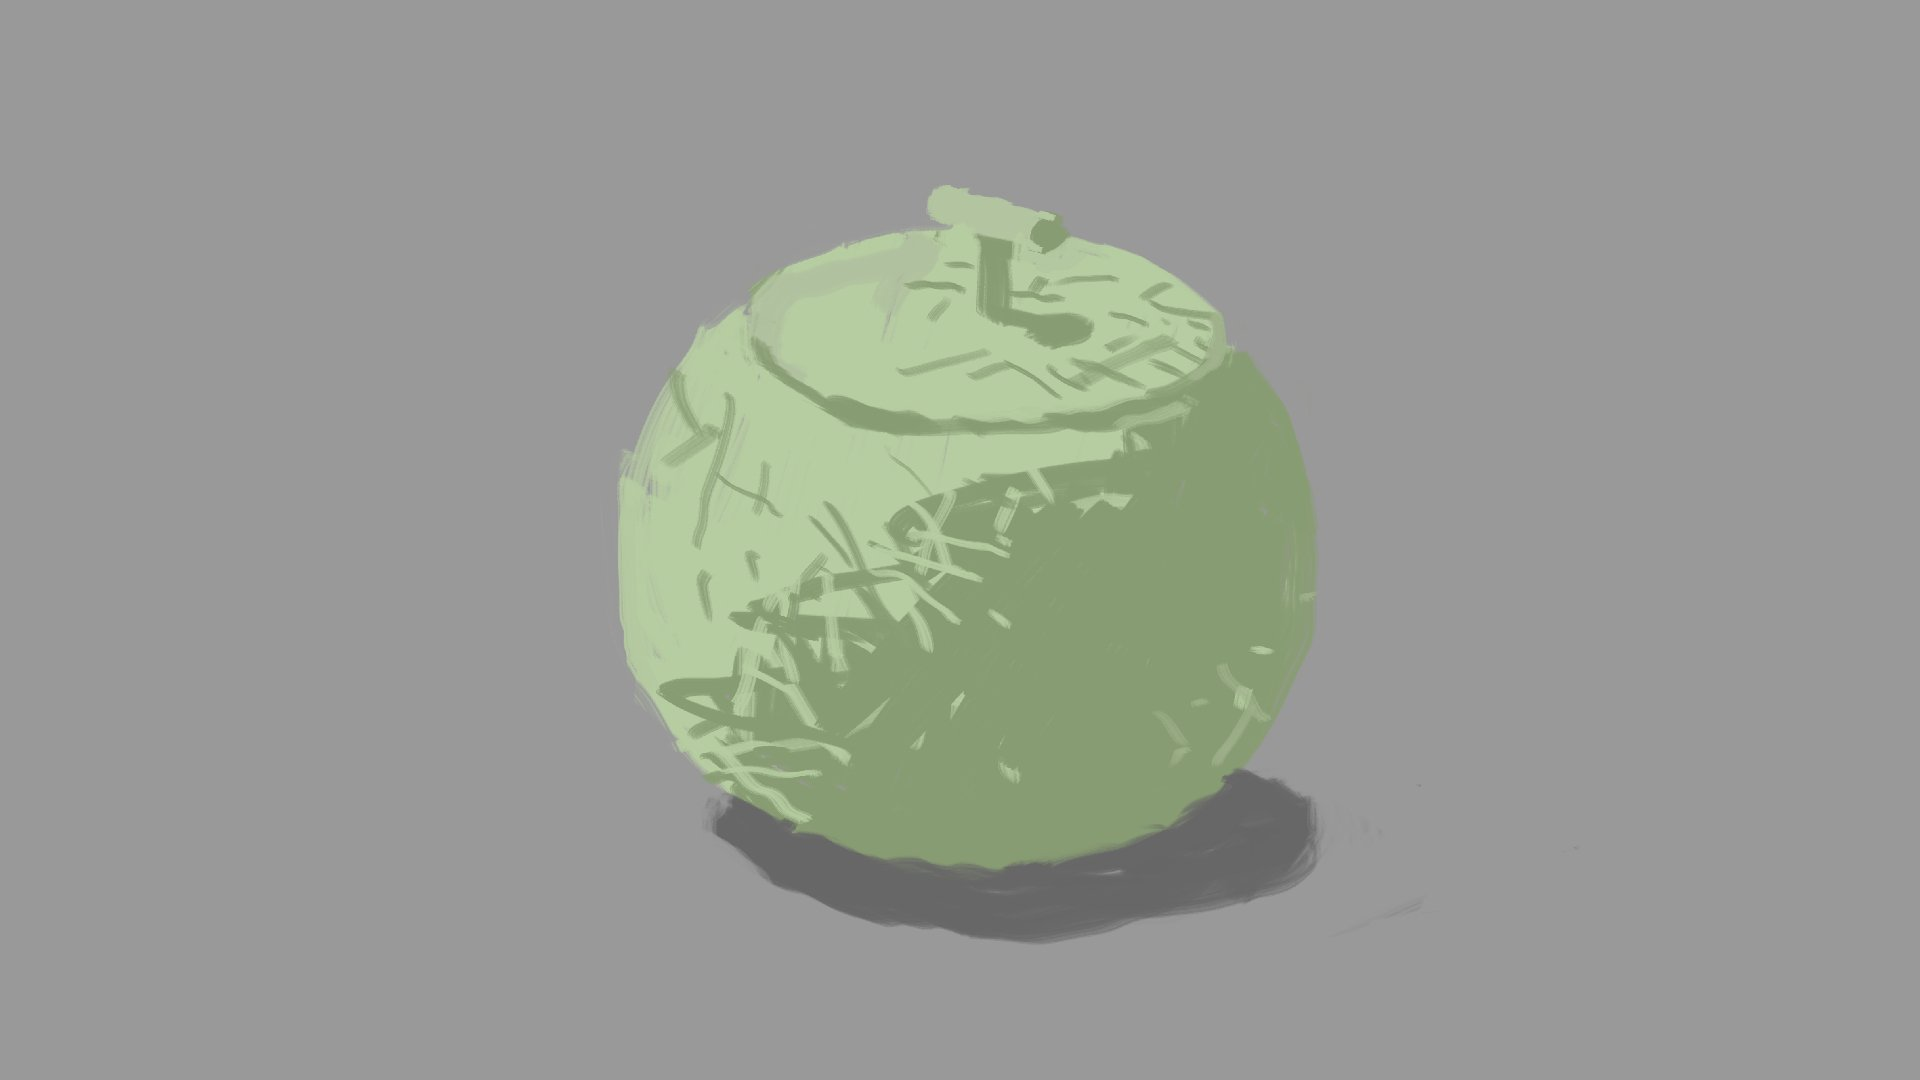
\includegraphics[scale=0.1]{melon.jpg}
\caption{Cucumis melo}
\end{figure}

\newpage
\section{Integrating over Non-Rectangular Regions}
\begin{figure}[h!]
    \centering
    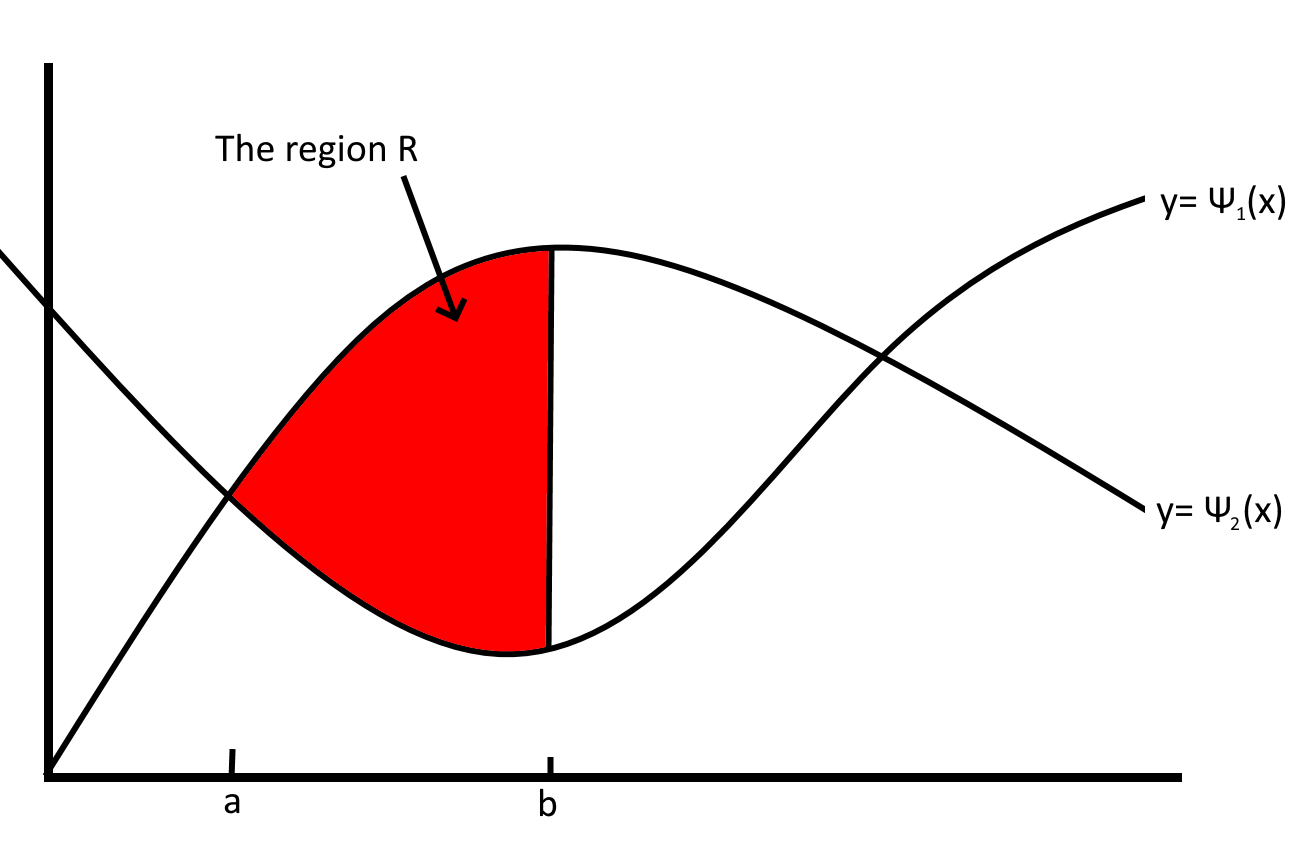
\includegraphics[scale=.2]{rectRegion.png}
    \caption{}
    \label{}
\end{figure}
$f(x,y)$ is a continuous function
\[\iint_R f(x,y)dydx =\int^a_b \int^{\Psi_2 (x)}_{\Psi_2 (x)}f(x,y)dydx\]

\begin{figure}[h!]
    \centering
    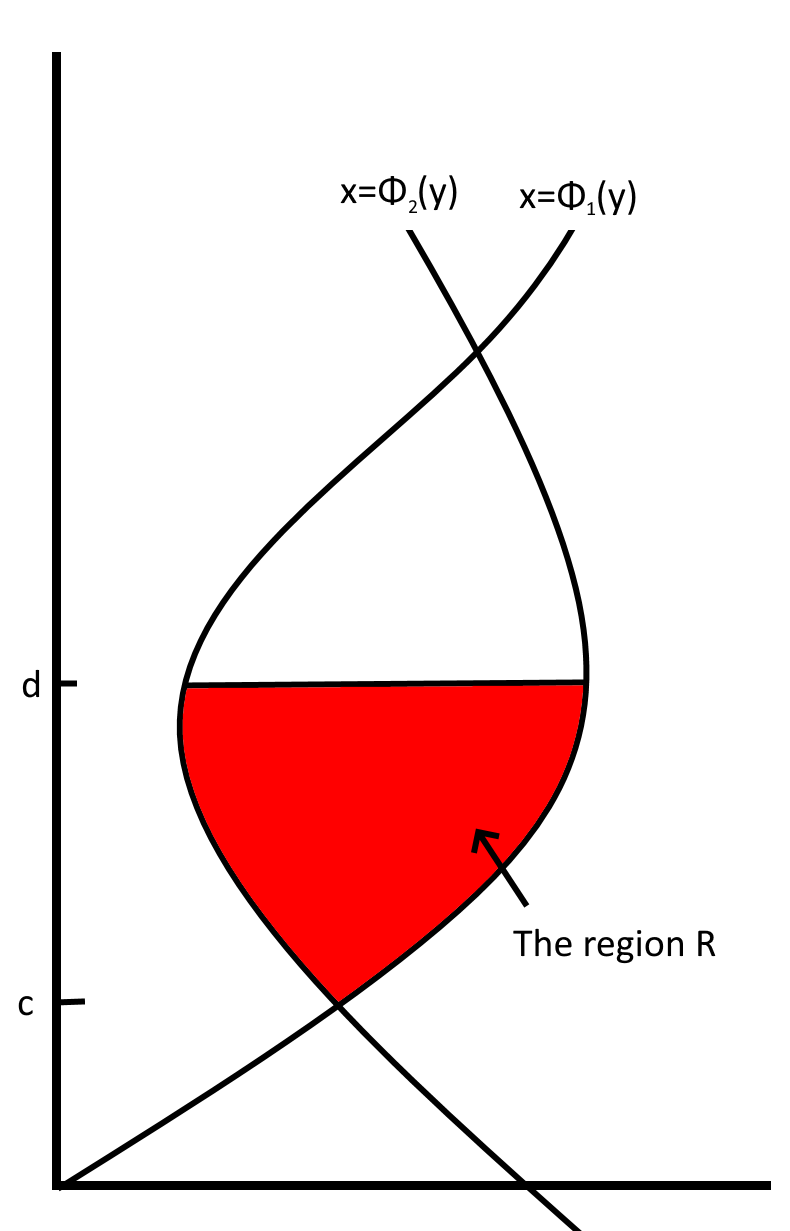
\includegraphics[scale=.2]{rectRegion2.png}
    \caption{}
    \label{}
\end{figure}

\[\iint_R f(x,y)dydx=\int^d_c \int^{\Phi_{2}(y)}_{\Phi_1 (x)} f(x,y)dxdy\]

\section{Switching the Order of Integration}
On a non-rectangular region, you have to be careful.
\begin{figure}[h!]
    \centering
    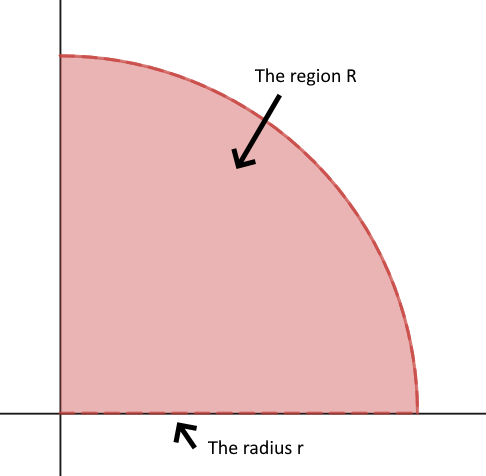
\includegraphics[scale=.5]{quarterCircle.png}

    \caption{Quarter Circle of $y=\sqrt{r^2-x^2}$}
    \label{}
\end{figure}
There are two ways to integrate $f(x,y)$ over R.
\begin{enumerate}
    \item $\int^r_0 \int^{\sqrt{r^2-x^2}}_0 f(x,y) dydx$
    \item $\int^r_0 \int^{\sqrt{r^2-y^2}}_0 f(x,y) dxdy$
\end{enumerate}

To switch the order of integration,
\begin{enumerate}
    \item Draw the region,
    \item Figure out how to describe the other way
\end{enumerate}

\subsection*{Example}
Evaluate:
\[\int^r_0\int^{\sqrt{r^2-x^2}}_0 \sqrt{r^2-y^2}dydx\]

Switch the order
\[=\int^r_0\int^{\sqrt{r^2-y^2}}_0 \sqrt{r^2-y^2}dxdy\]
\[=\int^r_0 \sqrt{r^2-y^2}\cdot \int^{\sqrt{r^2-y^2}}_0 1dydx = \int^r_0 \sqrt{r^2-y^2}\cdot\sqrt{r^2-y^2}dy\]
\[=\int^r_0 (r^2-y^2)dy\]
\[=r^3-\frac{r^3}{3}=\frac{2}{3}r^3\]

\subsection*{Exercise}
Evaluate $\int^1_0\int^1_x xydydx$

Switch the order and evaluate.

\[\int^1_0\int^1_y xydxdy =\int^1_0 \left[\frac{x^2 y}{2}\right]^1_y dy\]
\[=\int^1_0 (\frac{y}{2}-\frac{y^3}{2})dy = \left[\frac{y^2}{4}-\frac{y^4}{8}\right]^1_0=\frac{1}{8}\]

\end{document}